\chapter{METHODS AND RESULTS}

    In this section, finite element method (FEM) simulation results will be presented. The simulations are carried out on COMSOL Multiphysics V6.3 in RF Module physics. In this physics interface, the boundary conditions contained are perfect magnetic wall (PMW) and scattering boundary condition.
    
	\section{2D Microwave Mode Simulations}    
    
	Microwave mode simulations in 2D cross-section, as seen in Figure \ref{fig:microwave2D_wang-et-al}, consists of derivation of microwave mode index and characteristic impedance calculation for that mode. By using these parameters and optical mode index additionally, modulation bandwidth of modulator is calculated to predict high-speed capabilities of the device.
    
    \subsubsection{Microwave Mode Index  and Characteristic Impedance Parameter Sweeps For $w_{gap}$ \& $w_{pos}$}
    
    Dimensions given in the paper \cite{14} is taken as reference for beginning. These dimensions are seen in Table \ref{table:wang-et-al}. Then, microwave mode index is calculated by parametric simulations to find best matching for optical mode index, reference characteristic impedance value, 50Ohm by convention. Different than in the paper \cite{14}, electrode width $\omega _{pos}$ and gap $\omega _{gap}$ is simulated to design CPW.
    
    
    \begin{figure}[h!]
    	\begin{minipage}{0.5\textwidth}
    			\centering
    			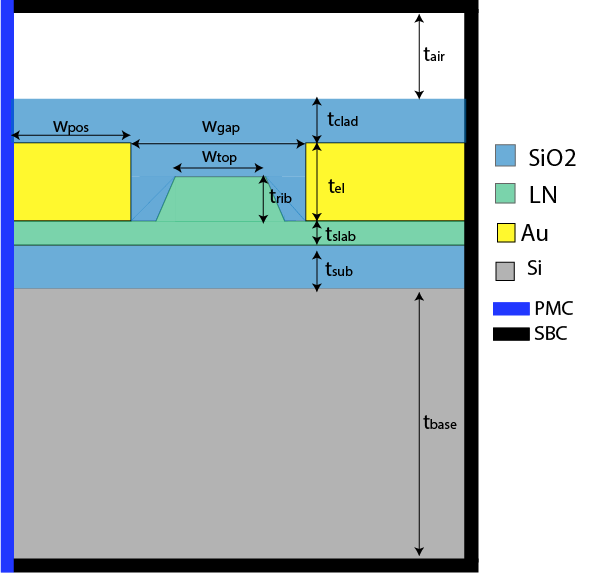
\includegraphics[width=0.85\linewidth]{simulation geometry.png} % replace with your image
    			\caption{Simulated Geometry}
    		\label{fig:microwave2D_wang-et-al}
		\end{minipage}%
\hfill
    \begin{minipage}{0.55\textwidth}
        \centering
        \begin{tabular}{|c|c|}
            \hline
            Property Name & Value  \\ \hline
            Air Thickness $(t_{air})$ & 10 $\mu m $  \\ \hline
            Cladding Thickness $(t_{clad})$ & 0.8 $\mu m $   \\ \hline
            Electrode Thickness $(t_{el})$ & 1.1 $\mu m $   \\ \hline
            Rib Thickness $(t_{rib})$ & 0.3 $\mu m $   \\ \hline
            Slab Thickness $(t_{slab})$ & 0.3 $\mu m $   \\ \hline
            Substrate Thickness $(t_{sub})$ & 4.7 $\mu m $  \\ \hline
            Base Thickness $(t_{base})$ & 500 $\mu m $    \\ \hline
            Positive Electrode Width $(w_{pos})$ & 4 $\mu m $  \\ \hline
            Gap $(w_{gap})$ & 9.895 $\mu m $    \\ \hline
            Rib Top Width $(w_{top})$ & 0.8 $\mu m $    \\ \hline
            $V_\pi L$ & 2.4115V    \\ \hline
        \end{tabular}
        \captionof{table}{Properties of simulated structure \cite{14}}
        \label{table:wang-et-al}
    \end{minipage}
\end{figure}
   

    In the Table \ref{table:wang-et-al}, calculated $V_{\pi}.L$ value and corresponding dimensions are given. In this work, $V_\pi L$ product is calculated via Equation (\ref{eq:vpiL-calculation_on_matlab}) on COMSOL-MATLAB Livelink interface. $V_{\pi}L$ value given in the paper \cite{14} is 2.3V. The error in calculation of $V_{\pi}L$ value is 4.8\%. In the Figure \ref{fig:microwave2D_wang-et-al}, the general simulation details are seen. Blue line on the left edge of geometry was included to mirror the structure to the left and PMC stands for perfect magnetic conductor. Remaining edges indicated with black lines demonstrate scattering boundary condition (SBC) to obtain results similar to real world behavior. That boundary is transparent for scattered waves.
    
    
   	
	
	\begin{figure}[h!]
        \centering
        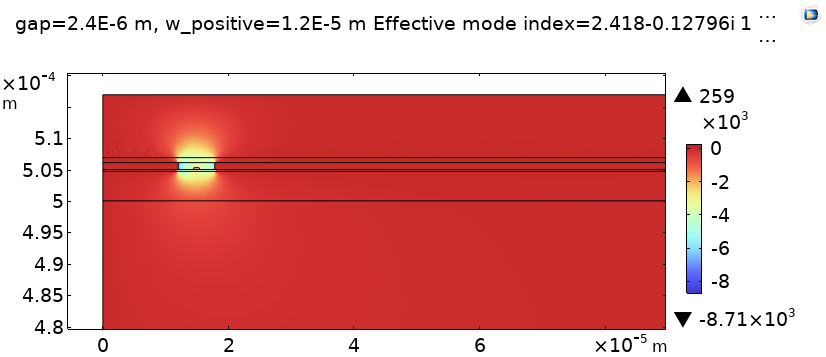
\includegraphics[width=0.8\linewidth]{field_overview_wpos_12um_gap_2.45um.png}
        \caption{Microwave field distribution in the CPW slot at 50GHz}
        \label{fig:cpw field distribution}
    \end{figure}
    
	In Figure \ref{fig:cpw field distribution}, one of the simulation result of microwave electric field's x-component is seen indicating the field confinement area. 	
	
	The aim at this point is to pinpoint microwave mode index and characteristic impedance of the transmission line. In Section \ref{sec:coplanar_waveguide}, the parameters which determines mode index characteristics and characteristic impedance are given. In this simulation, positive electrode width ($\omega _{pos}$) and gap ($\omega _{gap}$) are critical.
	

	Dynamic relation between $w_{pos}$, $w_{gap}$ and effective mode index is seen in Figure \ref{fig:index-change_colormap}. Based on this data and Equation (\ref{eq:neff_to_ng}), microwave group index is calculated. The data is seen in Figure \ref{fig:index-change_colormap} is obtained at 50GHz and additional simulation had been carried out at 55Ghz so that group index value is derived. 	
	
	\begin{equation}
		n_{el} = n_{eff} + f_{el} \pdv{n_{eff}}{f_{el}}
		\label{eq:neff_to_ng}
	\end{equation}   
	
	\newpage    
    % ------------------
	%\begin{figure}[h!]
    %    \centering
    %    \includegraphics[width=0.65\linewidth]{effective index colormap.png}
    %    \caption{Microwave mode index change color map based on $w_{gap}$ and $w_{pos}$ }
    %    \label{fig:index-change_colormap}
    %\end{figure}    
    % ------------------
	Increase of positive electrode width triggers an increase at the real part of microwave mode index and the increase of gap between electrodes causes decrease of microwave group index in Figure \ref{fig:index-change_colormap}. 
	
	 %\begin{figure}[h!]
     %	\begin{minipage}{0.5\textwidth}
     %			\centering
    %		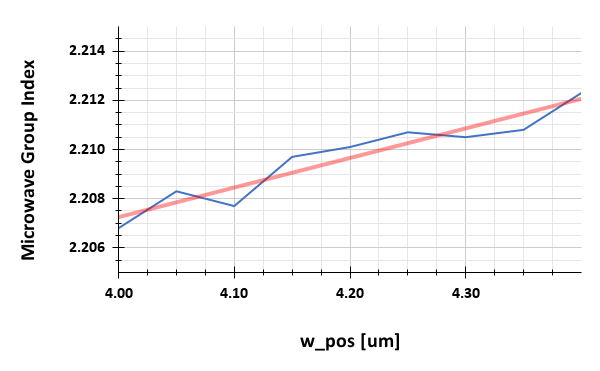
\includegraphics[width=0.85\linewidth]{microwave_group_index_w-pos.png}
    %			\caption{Simulated Geometry}
    %		\label{fig:ng_wpos}
	%	\end{minipage}%
	%	\hfill
    %	\begin{minipage}{0.55\textwidth}
    %    	\centering
     %   	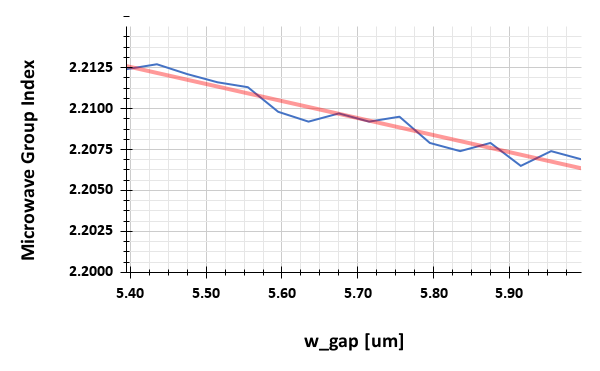
\includegraphics[width=0.85\linewidth]{microwave_group_index_gap.png}
      %  	\caption{Properties of simulated structure \cite{14}}
       % 	\label{fig:ng_wgap}
    	%\end{minipage}
	%\end{figure}
	
    As for the characteristic impedance of the line, calculations are based on the formula 
    
    \begin{equation}
    	Z_0 = \frac{V_o^2}{2P_{z-avg}}
    	\label{eq:experimental_char_imp}
    \end{equation}
    
    where $V_o$ is derived by the line integral of $E_x$ field along the gap between metal electrodes and $P_{z-avg}$ is time-average power integral into the geometry. Surface integral area is on the whole surface except metals electrodes. 
    
    For characteristic impedance calculation in Equation (\ref{eq:experimental_char_imp}), power term is multiplied by 2 and this indicates double the power obtained from simulations geometry given in Figure \ref{fig:microwave2D_wang-et-al}. In order to reduce simulation complexity, the geometry is divided by 2 and this halves the surface area which power integral is taken.
	% ------------------
    %\begin{figure}[h!]
    %    \centering
    %    \includegraphics[width=0.65\linewidth]{characteristic impedance colormap.png}
    %    \caption{Characteristic impedance change color map based on $w_{gap}$ and $w_{pos}$ }
    %    \label{fig:impedance-change_colormap}
    %\end{figure}
    % ------------------
    As the distance between two electrodes increases, per-unit-length-capacitance of the transmission line decreases.  Decrease of capacitance will lead to larger characteristic impedance as it is seen in Equation (\ref{eq:characteristic_impedance}). 
    
\subsubsection{Frequency Dependence CPW Parameters And Effects On Modulation Bandwidth}
    
	Frequency dependence of the two critical parameters are simulated. In Figure \ref{fig:ng_freq} and \ref{fig:Z0_freq} indicate the reason of band limitation on the response of waveguide-based electro-optic modulators. Eventually, the aim is having a index matching and impedance matching for larger frequency range. 
	
    % ------------------
	%\begin{figure}[h!]
    % 	\begin{minipage}{0.5\textwidth}
    % 			\centering
    %		\includegraphics[width=1\linewidth]{Microwave Group Index As A Function Of Frequency.png}
    %			\caption{Microwave group index \\ change depending on frequency}
    %		\label{fig:ng_freq}
	%	\end{minipage}%
	%	\hfill
    %	\begin{minipage}{0.5\textwidth}
    %    	\centering
    %    	\includegraphics[width=1\linewidth]{characteristic_impedance_vs_frequency_change.png}
    %    	\caption{Characteristic impedance change depending on frequency}
    %   	\label{fig:Z0_freq}
    %	\end{minipage}
	%\end{figure}    
	% ------------------
	
	In Figure \ref{fig:modulation_index_1}, bandwidth of non-optimized modulator is limited to 36GHz. 
    
	\begin{figure}[h!]
		\centering
        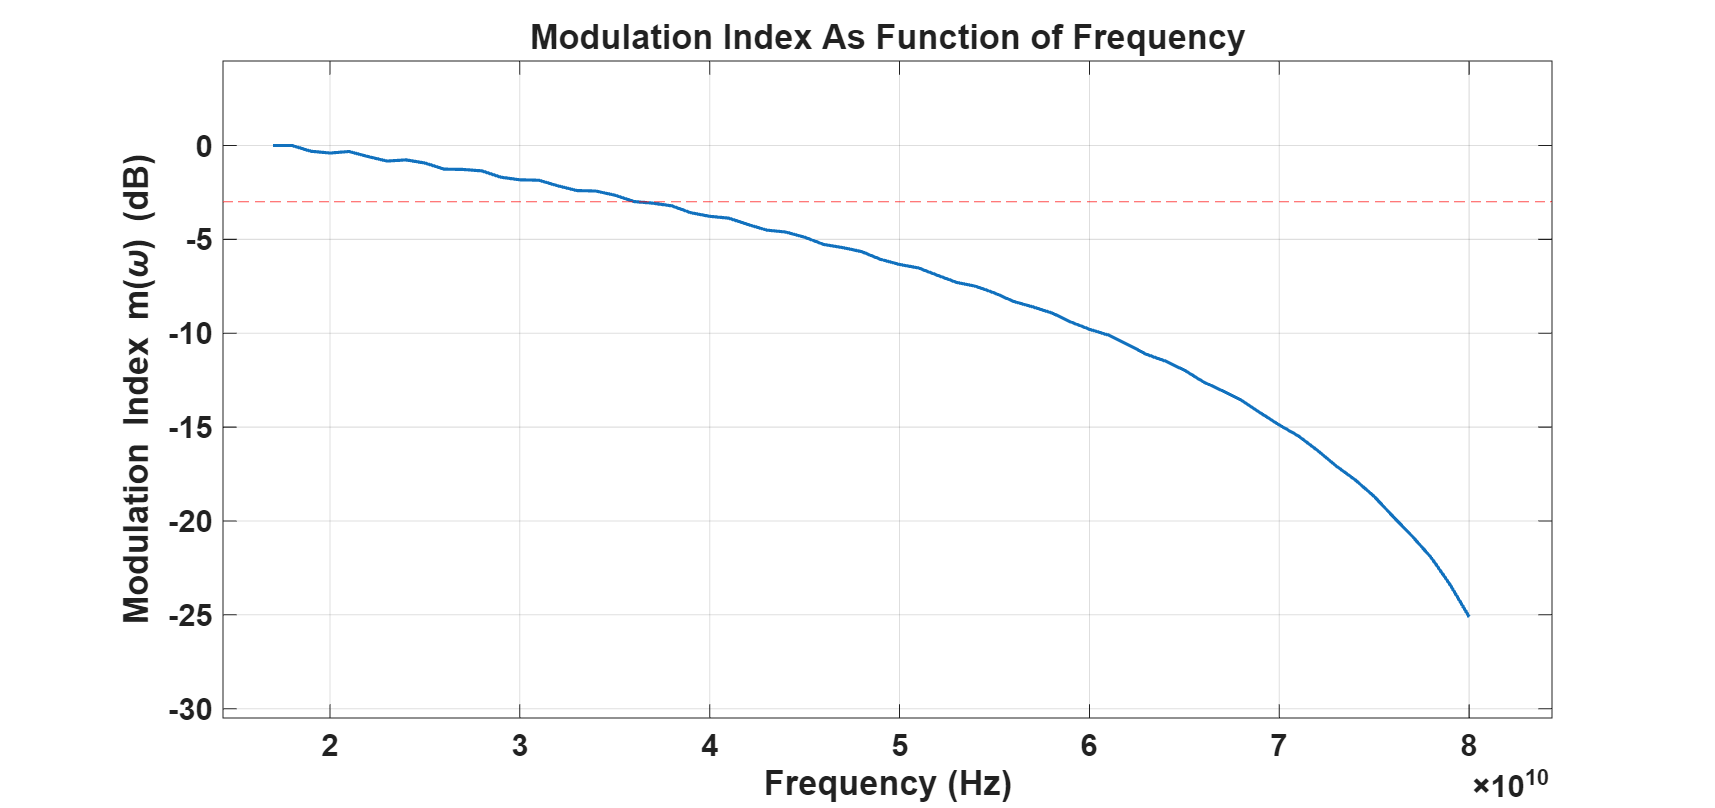
\includegraphics[width=0.9\linewidth]{modulation_index_vs_freq_15-80ghz_1ghz_step.png}
        \caption{Modulation index of the modulator geometry given in Figure \ref{fig:microwave2D_wang-et-al}. Calculation is based on the formula as in Equation (\ref{eq:eo-response})}
        \label{fig:modulation_index_1}
	\end{figure}	    
    
\subsubsection{T-Sections}
  	

   
    
    